\documentclass{article}
% translate with >> pdflatex -shell-escape <file>

% This file is an extract of the PGFPLOTS manual, copyright by Christian Feuersaenger.
% 
% Feel free to use it as long as you cite the pgfplots manual properly.
%
% See
%   http://pgfplots.sourceforge.net/pgfplots.pdf
% for the complete manual.
%
% Any required input files (for <plot table> or <plot file> or the table package) can be downloaded
% at
% http://www.ctan.org/tex-archive/graphics/pgf/contrib/pgfplots/doc/latex/
% and
% http://www.ctan.org/tex-archive/graphics/pgf/contrib/pgfplots/doc/latex/plotdata/

\usepackage{pgfplots}
\pgfplotsset{compat=newest}

\pagestyle{empty}

\begin{document}
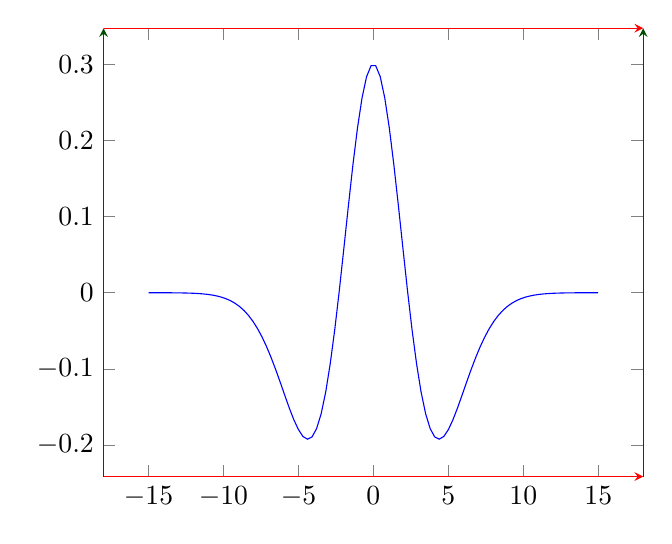
\begin{tikzpicture}
\begin{axis}[
	separate axis lines,
	every outer x axis line/.append style=
		{-stealth,red},
	every outer y axis line/.append style=
		{-stealth,green!30!black},
]
\addplot[blue,
		samples=100,
		domain=-15:15] 
	{1.3*exp(0-x^2/10) - exp(0-x^2/20)};
  % Unfortunately, there is a bug in PGF 2.00
  % something like exp(-10^2)
  % must be written as exp(0-10^2) :-(
\end{axis}
\end{tikzpicture}
\end{document}
